\documentclass[a4paper,12pt]{exam}
	\usepackage{graphicx}
	\usepackage[utf8]{inputenc}
	\usepackage[T1]{fontenc}
	\usepackage{listings}
	\usepackage{color}
	\usepackage{amsmath}
	\usepackage{enumerate}
	\usepackage{caption}
	\usepackage{subcaption}
	\definecolor{dkgreen}{rgb}{0,0.6,0}
	\definecolor{gray}{rgb}{0.5,0.5,0.5}
	\definecolor{mauve}{rgb}{0.58,0,0.82}

	\lstset{frame=tb,
	  language=Python,
	  aboveskip=3mm,
	  belowskip=3mm,
	  showstringspaces=false,
	  columns=flexible,
	  basicstyle={\small\ttfamily},
	  numbers=none,
	  numberstyle=\tiny\color{gray},
	  keywordstyle=\color{blue},
	  commentstyle=\color{dkgreen},
	  stringstyle=\color{mauve},
	  breaklines=true,
	  breakatwhitespace=true
	  tabsize=3
	}

\begin{document}
	\begingroup 
	  \bf Mecânica Clássica I - Resolução do exercício 3 da primeira prova\\
	  \indent André Del Bianco Giuffrida
	\endgroup
	\\ 
	\\ 
	\indent \textit{ Uma partícula de massa $m$ está sujeita a uma força:}
		$ \vec{F}(r)= -\frac{\beta}{r^3}\hat{r} $ \textit{ onde $\beta$ é uma constante positiva.}
		
		\[ V(\infty) - V(r) = - \int_{r}^{\infty} F(r')dr' = \int_{r}^{\infty} \frac{\beta}{r'^3} dr' = -\frac{\beta}{2r'^2} \Bigg|_{r}^{\infty} = +\frac{\beta}{2r^2}\]
		
		 \[\quad \text{Como $V(\infty) = 0$ obtemos que o potencial da força é dado por:} V(r) = -\frac{\beta}{2r^2} \]
		
		\[ \text{O Potencial fetivo é:} \quad V_{ef} = \frac{ L^2 }{2mr^2} - \frac{\beta}{2r^2}  = \frac{1}{2r^2} \Bigg[\frac{L^2}{m} - \beta \Bigg] \]
		
		Partindo de $\vec{F} = m\vec{a}$ temos $-\frac{\beta}{r^3}\hat{r} = m \big(\ddot{r} - r\dot{\theta}^2 \big)\hat{r} $ , ou seja, $ \ddot{r} - \frac{L^2}{m^2 r^3} = -\frac{\beta}{mr^3}$ com isso obtemos a seguinte equação:
		
		\[ m\ddot{r} = \frac{L^2}{mr^3} - \frac{\beta}{r^3} \quad \text{
		Usando os mesmos truques da gravitação, } \quad \frac{d^2u}{d\theta^2}  = u \Big( \frac{\beta m}{L^2} - 1 \Big) \]
		a solução aqui fica $ u(\theta) = Acos(\omega \theta - \varphi) $ onde $u=\frac{1}{r}$ e assim conseguimos a equação geral para o movimento:
		\[ r(\theta) = \frac{1}{Acos(\omega \theta - \varphi)} \quad \text{para} \quad \omega = \sqrt{\frac{\beta m}{L^2} - 1} \quad \text{ e } A = \sqrt{\frac{\frac{L^2}{m} - \beta}{2E}}\]
		\[ r(\theta) = \frac{\sqrt{\frac{2E}{\beta}}}{cos( \theta \sqrt{\frac{\beta m}{L^2} - 1} ) \sqrt{\frac{L^2}{\beta m} - 1}  } \]
		Isso nos leva aos possíveis movimentos:
		\begin{figure}[h]
			\centering
			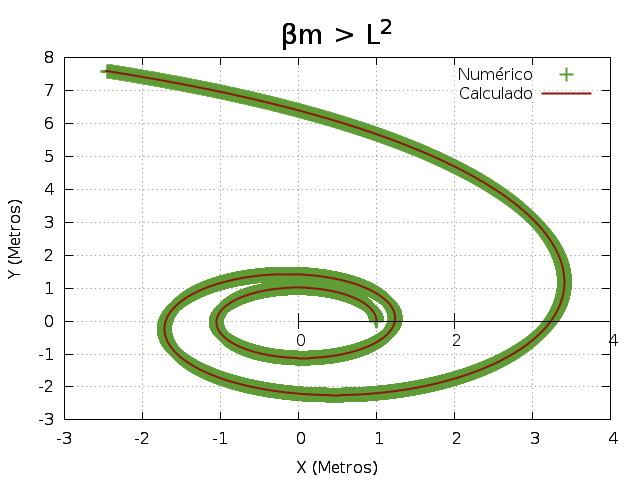
\includegraphics[scale=0.23]{3o0.png}
			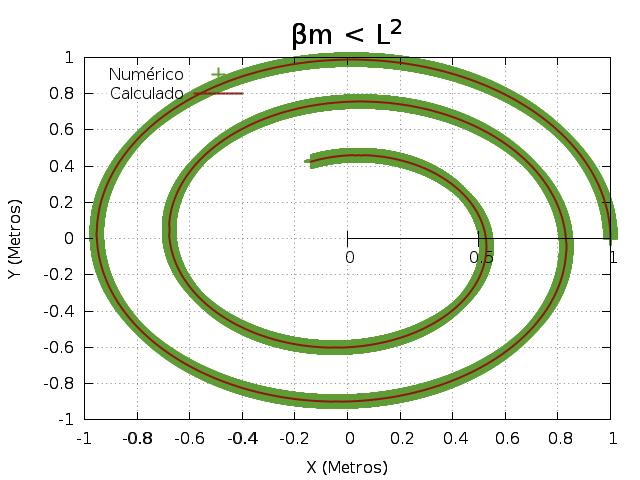
\includegraphics[scale=0.23]{3o1.png}
			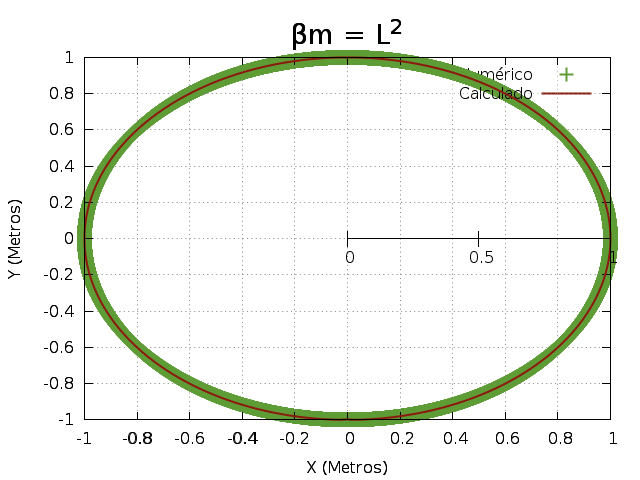
\includegraphics[scale=0.23]{3o3.png}
		\end{figure}
		
	\end{document}
